
\section{Module 1: Production of Power from Heat}


\subsection{Review of Thermodynamics}

\begin{enumerate}

%%%
%%%
%%%
\item {\it Given  Ar at P$_{1}$ = 140 kPa, T$_{1}$ = 10$^{o}$C, V$_{1}$ = 200 liters which undergoes a polytropic compression to P$_{2}$ = 700 kPa, T$_{2}$ = 180 $^{o}$C, find Q$_{1}^{2}$.}


In order to calculate Q$_{1}^{2}$, we will need to invoke the first law,
\begin{displaymath}
U_{2} - U_{1} = Q_{1}^{2} - W_{1}^{2} 
\end{displaymath}
For ideal gases, we need to calculate $\Delta U$ (based on $\Delta T$) and we can easily compute $W_{1}^{2}$ from its definition as $\int\limits_{1}^{2}PdV$. Using the following data for noble gas {\it Ar}:
\begin{displaymath}
MW\footnote{MW: Molecular weight; R: Universal gas constant; C$_{v}$: Heat capacity at constant volume.}=39.948 kg.\left(kmole\right)^{-1}\;\;\;\; R=0.2081 kJ.\left(kg.K\right)^{-1}\;\;\;\;C_{v}=0.312 kJ.\left(kg.K\right)^{-1}
\end{displaymath}
The mass of {\it Ar} can be calculated from state 1:
\begin{displaymath}
m=\displaystyle\frac{P_{1}V_{1}}{RT_{1}}=\displaystyle\frac{ \left(140 kPa\right) \left(0.2 m^{3}\right) } { \left(0.2081 \displaystyle\frac{kJ}{kg.K}\right) \left(283.15 K\right)} = 4.75192\times 10^{-1} kg
\end{displaymath}

The volume at state 2 can be easily calculated as,
\begin{eqnarray}
&& P_{2}V_{2}=mRT_{2} \nonumber \\
&& V_{2} =\displaystyle\frac{ \left(4.75192\times 10^{-1} kg\right) \left(0.2081 \displaystyle\frac{kJ}{kg.K}\right) \left(453.15 K\right) } {700 kPa} = 6.40155 \times 10^{-2} m^{-3} \nonumber
\end{eqnarray}

For polytropic processes,
\begin{eqnarray}
&&P_{i}V_{i}^{n} = \text{constant} = C \nonumber \\
&&\displaystyle\frac{P_{1}}{P_{2}} = \left(\displaystyle\frac{V_{2}}{V_{1}}\right)^{n} \nonumber \\
&&\ln \left( \displaystyle\frac{P_{1}}{P_{2}} \right) = \ln \left(\displaystyle\frac{V_{2}}{V_{1}}\right)^{n} \nonumber \\
&& n = \displaystyle\frac{ \ln \left( \displaystyle\frac{P_{1}}{P_{2}} \right)  } { \ln \left(\displaystyle\frac{V_{2}}{V_{1}}\right) }  = 1.41279 \nonumber
\end{eqnarray}


So the work in polyprotic processes can be defined as,
\begin{eqnarray}
W_{1}^{2} = && \int\limits_{1}^{2}\displaystyle\frac{C}{V^{n}}dV = C \int\displaystyle\frac{dV}{V^{n}} \nonumber \\
           && \left.\displaystyle\frac{C}{1-n} V^{(1-n)} \right|_{1}^{2} = \displaystyle\frac{C}{1-n}  \left( V_{2}^{(1-n)}-V_{1}^{(1-n)}\right) \nonumber
\end{eqnarray}
As $C = P_{1}V_{1} = P_{2}V_{2}$,
\begin{displaymath}
W_{1}^{2} = \displaystyle\frac{P_{2}V_{2}-P_{1}V_{1}}{1-n} = -40.7251 kJ
\end{displaymath}


The work is negative $\Longrightarrow$ {\it Ar} was worked upon in compression. From the first law,
\begin{eqnarray}
&& U_{2} - U_{1} = Q_{1}^{2} - W_{1}^{2} \nonumber \\
&& Q_{1}^{2} = U_{2} - U_{1} + W_{1}^{2} \nonumber 
\end{eqnarray}
Assuming that {\it Ar} behaves like an ideal gas, \ie $u=u(T)$ $\left(\text{with }u=\displaystyle\frac{U}{m}\right)$, 
\begin{displaymath}
\displaystyle\frac{du}{dT} = C_{v}
\end{displaymath}
and hence,
\begin{eqnarray}
Q_{1}^{2} &=& mC_{v}\left(T_{2} - T_{1}\right) + W_{1}^{2} \nonumber \\
         &=& \left( 4.75192\times 10^{-1} kg \right) \left( 0.312 kJ.\left(kg.K\right)^{-1} \right) \nonumber \left( 453.15 K - 283.15 K \right) + \left( -40.7251 kJ \right) \nonumber \\
         &=& \textcolor{red}{-15.5209 kJ} \nonumber
\end{eqnarray}
The variation of heat (or heat transfer) is negative $\Longrightarrow$ heat was lost from the system although temperature increased. This is because the raise in internal energy was mainly due to work than by the heat exchanged.   

\begin{figure}[h]
\begin{center}
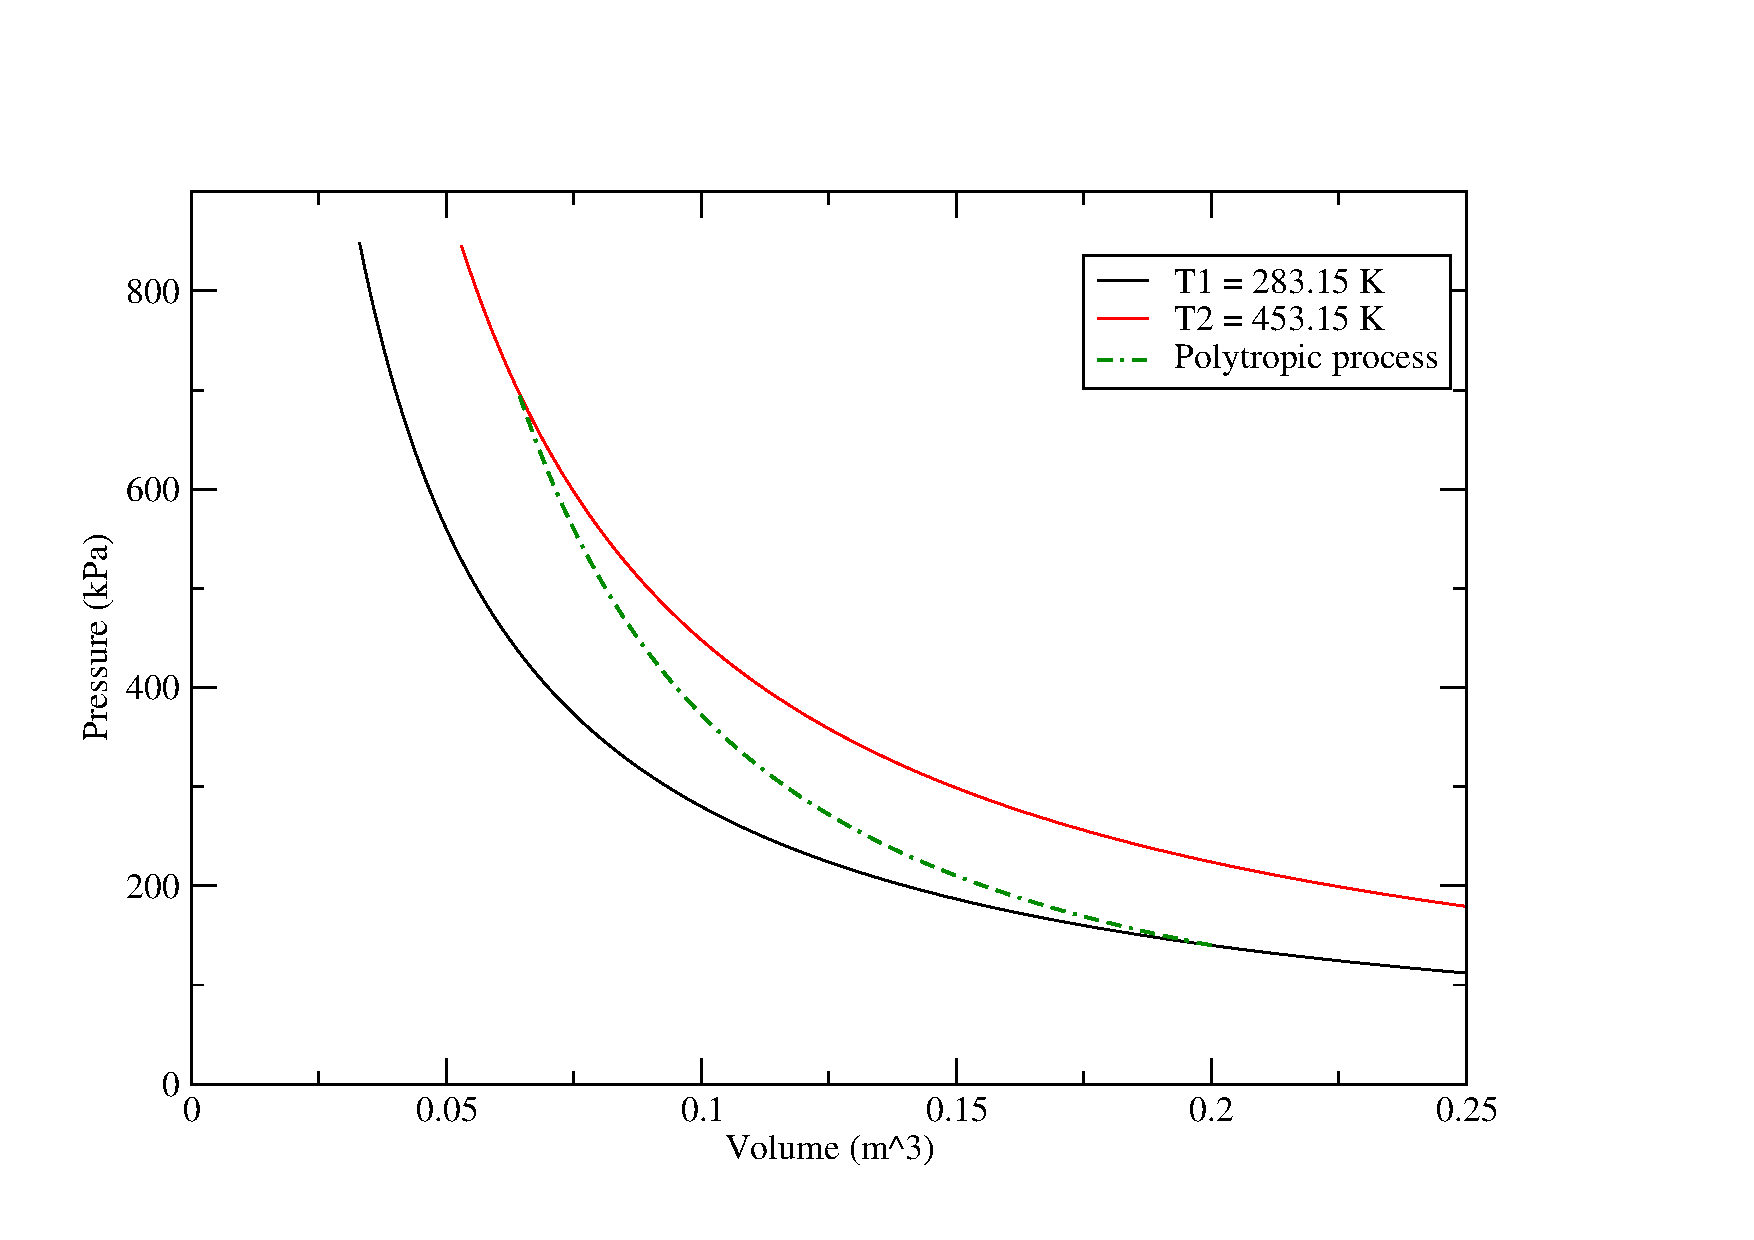
\includegraphics[width=13.0cm,height=8.0cm]{./../../ThermalEngines/Pics/example00_1}
\end{center}
\caption{Polytropic compression of {\it argonium} (green) from state 1 $\left(\text{V}_{1}=0.2 m^{3}\right)$ to 2 $\left(\text{V}_{2}=6.40\times 10^{-2}m^{3}\right)$. Ideal processes with isothermal temperature $T_{1}$ = 10 $^{o}$C (black) and $T_{2}$ = 180 $^{o}$C (red)}.
\end{figure}


%%%
%%%
%%%
\item {\it Given air (assuming ideal gas behaviour) expanding reversibly and adiabatically from $T_{1}=450 K$ and $V_{1}=3.0\times 10^{-3}m^{3}$ to the final volume, $V_{2}=5.0\times 10^{-3}m^{3}$. $T$ and $V$ relationship for constant heat capacities is represented by
\begin{displaymath}
\frc{T_{2}}{T_{1}} = \left(\frc{V_{1}}{V_{2}}\right)^{\gamma-1}
\end{displaymath}
(a) Derive a relationship between $T$ and $P$; Assuming that $C_{p}= 5.0 cal.\left(mol.K\right)^{-1}$ and $C_{v}=3.0 cal.\left(mol.K\right)^{-1}$, calculate (b) $T_{2}$, (c) the work done during the process and the (d) enthalpy change. }

The total energy change, $\Delta E$ can be split into
\begin{displaymath}
\Delta E = \Delta E_{K} + \Delta E_{P} + \Delta U = Q - W
\end{displaymath}
where $\Delta E_{K}$, $\Delta E_{P}$ and $\Delta U$ represent the change in kinetic, potential and internal energy, respectively. Assuming that the expansion process, the sum of the kinetic and potential energies of the system does not change,
\begin{displaymath}
\Delta E = \Delta U = Q - W
\end{displaymath}
or in differential form
\begin{displaymath}
dU = \delta Q - \delta W
\end{displaymath}
and all energy exchange with the surroundings are used to only change the internal energy. As the process is adiabatic ($Q=0$),
\begin{displaymath}
 dU = -\delta W = -P dV
\end{displaymath}
Since the gas is ideal, $dU=C_{v}dT = -PdV$ and,
\begin{displaymath}
V=\frc{RT}{P}
\end{displaymath}
and applying the chain rule to $V=V(T,P)$
\begin{displaymath}
dV = \frc{\partial V}{\partial T}dT + \frc{\partial V}{\partial P}dP= -\frc{RT}{P^{2}}dP + \frac{R}{P}dT
\end{displaymath}
 thus replacing $dV$,
\begin{displaymath}
C_{v}dT = - PdV = -P\left[-\frc{RT}{P^{2}}dP + \frc{R}{P}dT\right] = RT\frc{dP}{P} - RdT
\end{displaymath}
Since $C_{p}-C_{v}=R$ and replacing $C_{v}$ in the equation above,
\begin{displaymath}
C_{p}dT = RT\frc{dP}{P} \Longrightarrow \frc{dT}{T} = \frc{R}{C_{p}}\frc{dP}{P} \Longrightarrow \frc{dT}{T} = \frc{C_{p}-C_{v}}{C_{p}}\frc{dP}{P}=\left(\frc{\gamma - 1}{\gamma}\right)\frc{dP}{P}
\end{displaymath}
where $\gamma = C_{p}/C_{v}$. Integrating from state 2 to 1:
\begin{eqnarray}
&& \ln\frc{T_{2}}{T_{1}}=\left(\frc{\gamma - 1 }{\gamma}\right)\ln\frc{P_{2}}{P_{1}} \;\;\; \text{or} \nonumber \\
&& \textcolor{red}{\frc{T_{2}}{T_{1}} = \left(\frc{P_{2}}{P_{1}}\right)^{\frc{\gamma-1}{\gamma}}} \nonumber 
\end{eqnarray}

\medskip

Temperature, $T_{2}$ is obtained from 
\begin{eqnarray}
&& \frc{T_{2}}{T_{1}} = \left(\frc{V_{1}}{V_{2}}\right)^{\gamma - 1} \nonumber \\
&& T_{2} = T_{1} \left(\frc{V_{1}}{V_{2}}\right)^{\gamma - 1 } = (450\;K)\left[\frac{3.0\times 10^{-3}\;\;m^{3}}{5.0\times 10^{-3}\;\;m^{3}}\right]^{\left(\frc{5.0\;cal.\left(mol.K\right)^{-1} }{3.0\; cal.\left(mol.K\right)^{-1}  }-1\right)} \nonumber \\
&& \textcolor{red}{T_{2} = 320.12 K} \nonumber
\end{eqnarray}

The work done during the process is,
\begin{eqnarray}
&& W = -\Delta U = - C_{v}\Delta T = \left[ -3.0\; cal.\left(mol.K\right)^{-1} \right] \left( 320 - 450 \;\;K\right) \nonumber \\
&& \textcolor{red}{W = 390 \frc{cal}{mol} = 1632.85 \frc{J}{mol}} \nonumber
\end{eqnarray}
$W>0$ indicates that in the expansion process, work is done by the system. The enthalpy change of the gas can be calculated as,
\begin{eqnarray}
&& \Delta H = C_{p}\Delta T = \left[ 5.0\; cal.\left(mol.K\right)^{-1} \right] \left( 320 - 450 \;\;K\right) \nonumber \\
&& \textcolor{red}{\Delta H = -650 \frc{cal}{mol} = -2721.42 \frc{J}{mol}} \nonumber 
\end{eqnarray}


%%%
%%% Problems for the students:
%%%

%%%
%%% Problem 2.69 (Saphiro)
%%%
\item {\it Gaseous CO$_{2}$ $\left(\text{m}_{CO_{2}}=4g\right)$ is contained in a vertical piston-cylinder assembly by a piston of mass 50 kg and having a face area of 1.0$\times$10$^{-2}$m$^{2}$. The CO$_{2}$ initially occupies a volume of 5$\times$10$^{-3}$m$^{3}$ and has a specific internal energy of 657 kJ.kg$^{-1}$.  The atmosphere exerts a pressure of 100 kPa on the top of the piston. Heat transfer in the amount  of 1.95 kJ occurs slowly from the CO$_{2}$ to the surroundings, and the volume of the CO$_{2}$ decreases to 2.5$\times$10$^{-3}$m$^{3}$. Friction between the piston and the cylinder wall can be neglected. The local acceleration of gravity is 9.81 m.s$^{-2}$. For the CO$_{2}$, determine (a) the pressure in kPa and (b) the final specific internal energy in kJ.kg$^{-1}$.}

%%%
%%% Problem 2.33 (Saphiro)
%%%
\item {\it CO gas contained within a piston-cylinder assembly undergoes three processes in series:\\
       Process 1-2: expansion from p$_{1}$ = 5 bar, V$_{1}$ = 0.2 m$^{3}$ to V$_{2}$ = 1.0 m$^{3}$, during which the pressure-volume relationship is pV = constant.\\
       Process 2-3: constant volume heating from state 2 to state 3, where p$_{3}$ = 5 bar.\\
       Process 3-1: constant pressure compression to the initial state.\\
       Sketch the processes in series on p-V coordinates and evaluate the work for each process, in kJ.}

%%%
%%% Problem 2.61 (Saphiro)
%%%
\item {\it One kg of Refrigerant 22. initially at p$_{1}$ = 0.9 MPa, u$_{1}$ = 232.92 kJ/kg, is contained within a rigid closed tank The tank is fitted with a paddle wheel that transfers energy to the refrigerant at a constant rate of 0.1 kW. Heat transfer from the refrigerant to its surroundings occurs at a rate Kt, in kW, where K is a constant (in kW/min) and t is time (in min).  After 20 minutes of stirring the refrigerant is at p$_{2}$ = 1.2 MPa, u$_{2}$ = 276.67 kJ/kg. No overall changes in kinetic or potential energy occur. (a) For the refrigerant, determine the work and heat transfer; (b) determine value of the constant K (in kW/min).}

%%%
%%% Problem 2.89 (Saphiro)
%%%
\item {\it A household refrigerator operating steadily and with a coefficient of performance of 2.4 removes energy from a refrigerated  space at a rate of 600 Btu/h. Evaluating electricity at $\pounds$0.08 per kW.h, determine the cost of electricity in a month when the refrigerator operates for 360 hours.}

%%%
%%% Problem 2.90 (Saphiro)
%%%
\item {\it A heat pump cycle operating at steady state receives energy by heat transfer from well water at 10$^{o}$C and discharges energy by heat transfer to a building at the rate of 1.2$\times$10$^{5}$ kJ/h. Over a period of 14 days, an electric meter records that 1490 kW.h of electricity is provided to the heat pump. These are the only energy transfers involved.  Determine (a) the amount of energy that the heat pump receives over the 14-day period from the well water by heat transfer (in kJ), and (b) the heat pump's coefficient of performance.}


%%%
%%% Problem 2.36 (S&V)
%%%
\item {\it 1 kg of air is heated reversibly at constant pressure from an initial state of 300 K and 1 bar until its volume triples. Calculate W, Q, $\Delta$U, $\Delta$H for the process. Assume for air that
\begin{displaymath}
\frc{PV}{T} = 83.14 \;\;\; \frc{\text{bar.cm}^{3}}{mol}\;\;\;\;\;\text{and}\;\;\;\;\;C_{p}=29\frc{\text{J}}{\text{mol.K}}
\end{displaymath}
}

%%%
%%% Problem 2.37 (S&V)
%%%
\item  {\it The conditions of a gas change in a steady-flow process from 20 $^{o}$C and 1000 kPa to 60 $^{o}$C and 100 kPa. Devise a reversible non-flow process (any number of steps) for accomplishing this change of state, and calculate $\Delta$U and $\Delta$H for the process on the basis of 1 mol of gas. Assume for the gas that PV/T is constant, $C_{v}$ = (5/2)R, and $C_{p}$ = (7/2)R.}

%%%
%%% Problem 5.21-24 (Saphiro)
%%%
\item {\it A reversible power cycle receives 100 kJ by hear transfer from a hot reservoir at 327 $^{o}$C and rejects 40 kJ by heat transfer to a cold reservoir at $T_{cold}$. Determine:
\begin{enumerate}
\item The thermal efficiency;
\item The temperature $T_{cold}$;
\item Maximum theoretical thermal efficiency for any power cycle operating between hot and cold reservoirs at 602 $^{o}$C and 112 $^{o}$C, respecively;
\item Assuming that two power cycles -- PC$_{A}$ and PC$_{B}$, operate at the same thermal efficiency. PC$_{A}$ with hot and cold reservoir temperatures of 2000 K and 1000 K, respectively, and PC$_{B}$ with $T_{cold}$ an 500 K. Calculate $T_{hot}$.
\end{enumerate}
}

%%%
%%% Problem 5.78 (Saphiro)
%%%
\item \label{prob:5_78}{\it The pressure-volume diagram of a Carnot power cycle executed by an ideal gas with constant specific heat ratio $\kappa$ is shown in Fig. \ref{Prob_Saphiro_5.78}. Demonstrate that: (a) $V_{4}V_{2}=V_{1}V_{3}$, (b) $\frc{T_{2}}{T_{3}} = \left(\frc{P_{2}}{P_{3}}\right)^{\frc{\kappa - 1}{\kappa}}$ and (c) $\frc{T_{2}}{T_{3}}=\left(\frc{V_{3}}{V_{2}}\right)^{\kappa - 1}$}
\begin{figure}[h]
\begin{center}
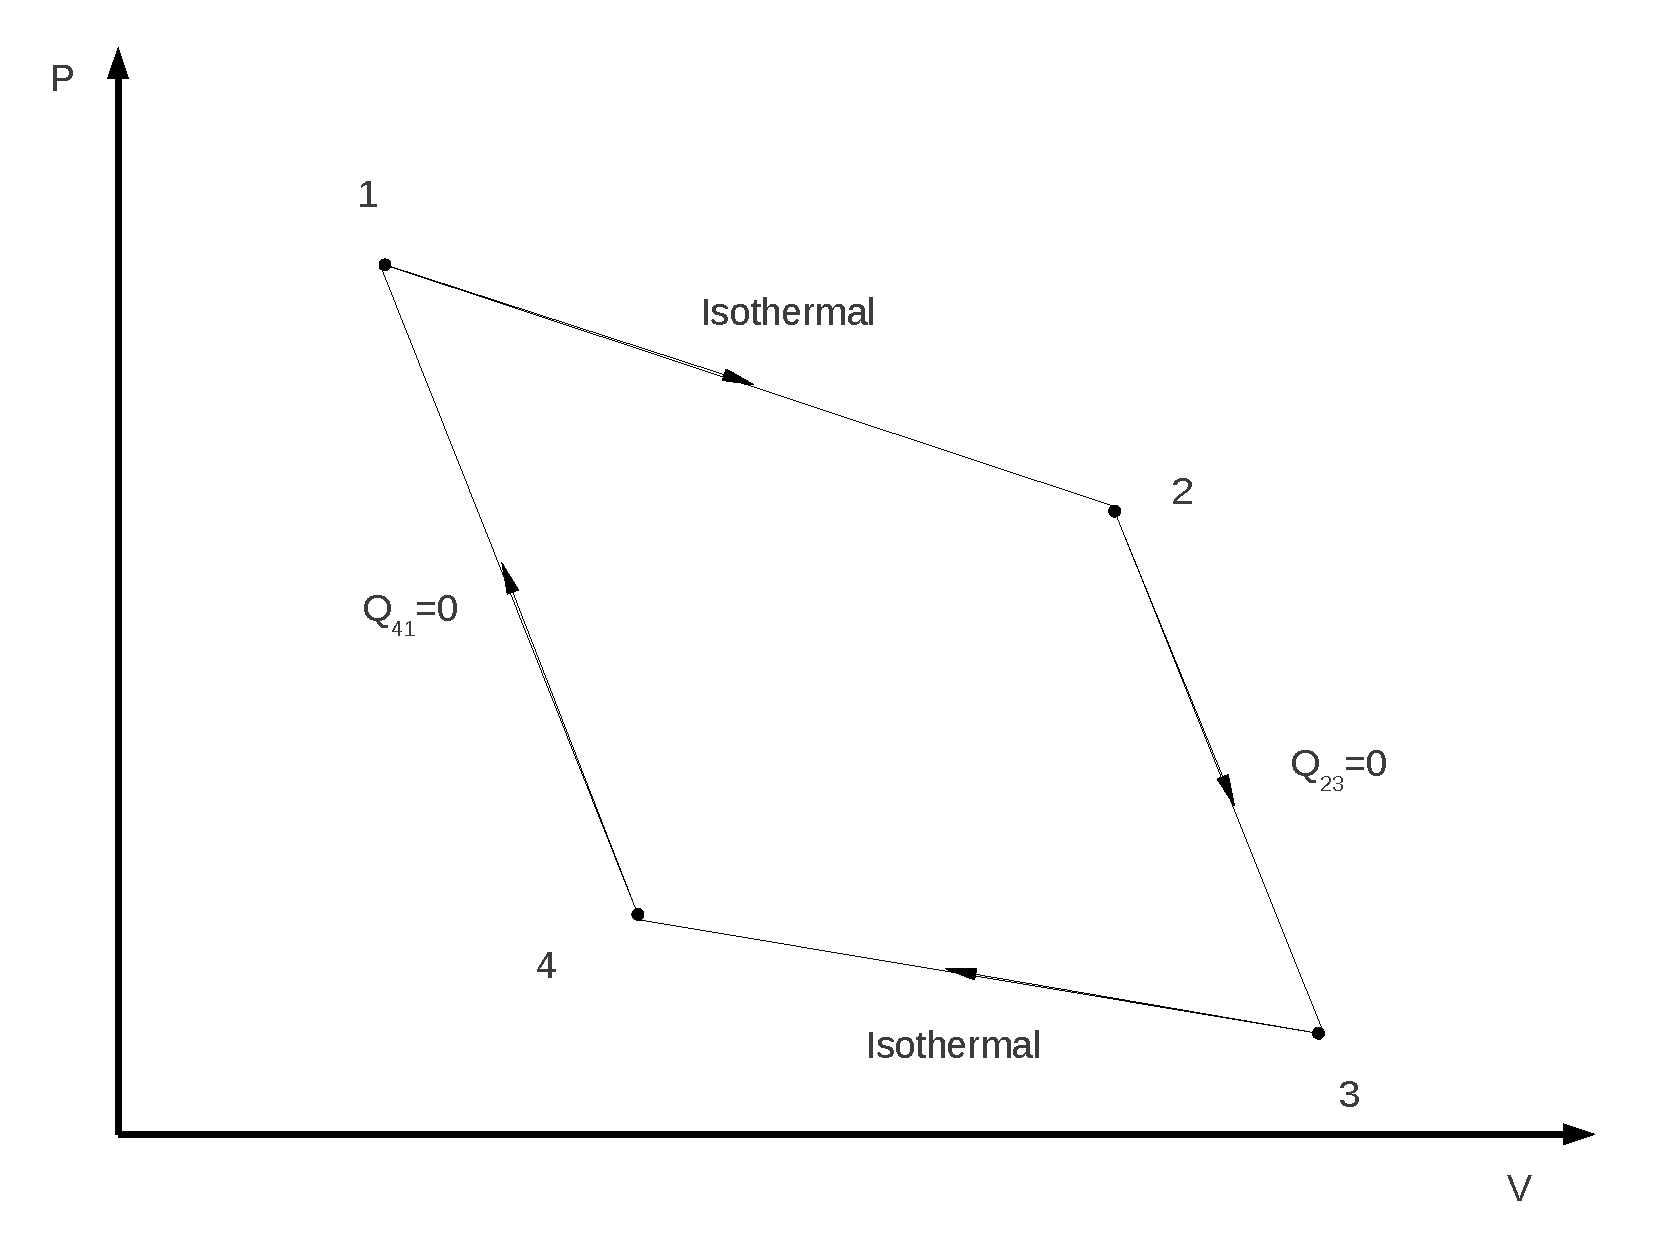
\includegraphics[width=15.cm,clip]{./../../ThermalEngines/Pics/Problem_5_78}
\caption{ \ref{prob:5_78}}
\label{Prob_Saphiro_5.78}
\end{center}
\end{figure}

%%%
%%% Problem 5.86 (Saphiro)
%%%
\item {\it A reversible refrigeration cycle $A$ and an irreversible refrigeration cycle $B$ operate between the same two reservoirs and each removes $Q_{c}$ from the cold reservoir. The net work input required by $A$ is $W_{A}$, while the net work input for $B$ is $W_{B}$. The reversible cycle discharges $Q_{H}$ to the hot reservoir, while the irreversible cycle discharges $Q^{\prime}_{H}$.  Using the Clausius inequality,, 
\begin{equation}
\oint\left(\frc{\delta Q}{T}\right) = - \sigma_{\text{cycle}} \label{eqn_clausius}
\end{equation}
show that $W_{B} > W_{A}$ and $Q^{\prime}_{H}>Q_{H}$. Using Eqn. \ref{eqn_clausius}, complete the following involving reversible and irreversible cycles:
\begin{enumerate}
\item Reversible and irreversible power cycles each discharge energy $Q_{C}$ to cold reservoir at temperature $T_{C}$ and receive energy $Q_{H}$ from hot reservoirs at temperatures $T_{H}$ and $T^{\prime}_{H}$, respectively. There are no other heat transfers in the system. Show that $T^{\prime}_{H}>T_{H}$.
\item Reversible and irreversible refrigeration cycles each discharge energy $Q_{H}$ to a hot reservoir at temperature $T_{H}$ and receive $Q_{C}$ from cold reservoirs at temperatures $T_{C}$ and $T^{\prime}_{C}$, respectively. There are no other heat transfer. Show that $T^{\prime}_{C}>T_{C}$.
\item Reversible and irreversible heat pump cycles each receive energy $Q_{C}$ from a cold reservoir at temperature $T_{C}$ and discharge energy $Q_{H}$ to hot reservoirs at temperatures $T_{H}$ and $T^{\prime}_{H}$, respectively. There are no other heat transfers. Show that $T^{\prime}_{H}<T_{H}$. 
\end{enumerate}
}

%%%
%%% Problem 5.7 (SM&VN)
%%%
\item {\it Large quantities of liquefied natural gas (LNG) are shipped by ocean tanker. At the unloading port provision is made for vaporisation of the LNG so that it may be delivered to pipelines as gas. The LNG arrives in the tanker at atmospheric pressure and 113.7 K, and represents a possible heat sink for use as the cold reservoir of a heat engine. For unloading of LNG as a vapour at the rate of 9000 $m^{3}.s^{-1}$, as measured at 298.15 K and 1.0133 bar, and assuming the availability of an adequate heat source at 303.15 K, what is the maximum possible power obtainable and what is the rate of heat transfer from the heat source? Assume that LNG at 298.15 K and 1.0133 bar is an ideal gas with the molar mass of 17. Also assume that the LNG vaporises only, absorbing only its latent heat of 512 kJ/kg at 113.7 K.}


%%%
%%% Problem 5.17 (SM&VN)
%%%
\item {\it A Carnot engine operates between temperature levels of 600 K and 300 K. It drives a Carnot refrigerator, which provides cooling at 250 K and discards heat at 300 K. Determine a numerical value for the ratio of heat extracted by the refrigerator ($\lq$cooling load') to the heat delivered to the engine ($\lq$heating load').}

%%%
%%% Problem 5.44 (SM&VN)
%%%
\item {\it A nuclear power plant generates 750 MW; the reactor temperature is 588.15 K and a river with water temperature of 293.15 K is available to provide system cooling. (a) What is the maximum possible thermal efficiency of the plant, and what is the minimum rate at which heat must be discarded to the river? (b)  If the actual thermal efficiency of the plant is 60$\%$ of the maximum, at what rate must heat be discarded to the river, and what is the temperature rise of the river if it has a flow rate of 165 $m^{3}/s$?}

%%%
%%% Problem 5.43 (SM&VN)
%%%
\item {\it Heat in the amount of 150 kJ is transferred directly from a hot reservoir at $T_{H} = 550 K$
to two cooler reservoirs at $T_{1} = 350 K$ and $T_{2} = 250 K$. The surroundings temperature is T, = 300 K. If the heat transferred to the reservoir at $T_{1}$ is half that transferred to the reservoir at $T_{2}$, calculate: (a) The entropy generation (in kJ/K); (b) The lost work ; (c) How could the process be made reversible?}


%%%
%%% Problem 8.3 (Power Lectures Notes)
%%%
\item {\it Given saturated ammonia vapour at $P_{1} = 200 kPa$ compressed by a piston to $P_{2} = 1.6 MPa$ in a
reversible adiabatic process, (a) find the work done per unit mass; (b) sketch the T-s and P-v diagrams.}

%%%
%%% Problem 8.5 (Power Lectures Notes)
%%%
\item {\it Given the enthalpy change (in water-steam thermodynamic table), calculate the entropy change for water going from saturated liquid to saturated vapour along a T = 100 ◦C isotherm.}


%%%
%%% Problem -- Callen
%%%
\item {\it Derive the Maxwell relations below,
\begin{displaymath}
%
 \left(\frac{\partial T}{\partial V}\right)_{s} = -\left(\frc{\partial P}{\partial s}\right)_{V} \;\;\;\;
%
 \left(\frc{\partial T}{\partial P}\right)_{s} = \left(\frac{\partial V}{\partial s}\right)_{P} \;\;\;\;
%
 \left(\frc{\partial P}{\partial T}\right)_{V} = \left(\frac{\partial s}{\partial V}\right)_{T} \;\;\;\;
%
  \left(\frac{\partial V}{\partial T}\right)_{P} = -\left(\frc{\partial s}{\partial P}\right)_{T} \;\;\;\; 
\end{displaymath}
from the fundamental thermodynamic equations,
\begin{eqnarray}
&& du = - PdV + Tds \nonumber \\ 
&& dh =   Tds + VdP \nonumber \\
&& df = - PdV - sdT \nonumber \\
&& dg = - VdP - sdT \nonumber
\end{eqnarray}}

\end{enumerate}
